% Options for packages loaded elsewhere
\PassOptionsToPackage{unicode}{hyperref}
\PassOptionsToPackage{hyphens}{url}
%
\documentclass[
]{book}
\usepackage{amsmath,amssymb}
\usepackage{lmodern}
\usepackage{iftex}
\ifPDFTeX
  \usepackage[T1]{fontenc}
  \usepackage[utf8]{inputenc}
  \usepackage{textcomp} % provide euro and other symbols
\else % if luatex or xetex
  \usepackage{unicode-math}
  \defaultfontfeatures{Scale=MatchLowercase}
  \defaultfontfeatures[\rmfamily]{Ligatures=TeX,Scale=1}
\fi
% Use upquote if available, for straight quotes in verbatim environments
\IfFileExists{upquote.sty}{\usepackage{upquote}}{}
\IfFileExists{microtype.sty}{% use microtype if available
  \usepackage[]{microtype}
  \UseMicrotypeSet[protrusion]{basicmath} % disable protrusion for tt fonts
}{}
\makeatletter
\@ifundefined{KOMAClassName}{% if non-KOMA class
  \IfFileExists{parskip.sty}{%
    \usepackage{parskip}
  }{% else
    \setlength{\parindent}{0pt}
    \setlength{\parskip}{6pt plus 2pt minus 1pt}}
}{% if KOMA class
  \KOMAoptions{parskip=half}}
\makeatother
\usepackage{xcolor}
\usepackage{longtable,booktabs,array}
\usepackage{calc} % for calculating minipage widths
% Correct order of tables after \paragraph or \subparagraph
\usepackage{etoolbox}
\makeatletter
\patchcmd\longtable{\par}{\if@noskipsec\mbox{}\fi\par}{}{}
\makeatother
% Allow footnotes in longtable head/foot
\IfFileExists{footnotehyper.sty}{\usepackage{footnotehyper}}{\usepackage{footnote}}
\makesavenoteenv{longtable}
\usepackage{graphicx}
\makeatletter
\def\maxwidth{\ifdim\Gin@nat@width>\linewidth\linewidth\else\Gin@nat@width\fi}
\def\maxheight{\ifdim\Gin@nat@height>\textheight\textheight\else\Gin@nat@height\fi}
\makeatother
% Scale images if necessary, so that they will not overflow the page
% margins by default, and it is still possible to overwrite the defaults
% using explicit options in \includegraphics[width, height, ...]{}
\setkeys{Gin}{width=\maxwidth,height=\maxheight,keepaspectratio}
% Set default figure placement to htbp
\makeatletter
\def\fps@figure{htbp}
\makeatother
\setlength{\emergencystretch}{3em} % prevent overfull lines
\providecommand{\tightlist}{%
  \setlength{\itemsep}{0pt}\setlength{\parskip}{0pt}}
\setcounter{secnumdepth}{5}
\usepackage{booktabs}
\ifLuaTeX
  \usepackage{selnolig}  % disable illegal ligatures
\fi
\usepackage[]{natbib}
\bibliographystyle{apalike}
\IfFileExists{bookmark.sty}{\usepackage{bookmark}}{\usepackage{hyperref}}
\IfFileExists{xurl.sty}{\usepackage{xurl}}{} % add URL line breaks if available
\urlstyle{same} % disable monospaced font for URLs
\hypersetup{
  pdftitle={DIYCGM},
  pdfauthor={https://personalscience.com},
  hidelinks,
  pdfcreator={LaTeX via pandoc}}

\title{DIYCGM}
\author{\url{https://personalscience.com}}
\date{2022-05-25}

\begin{document}
\maketitle

{
\setcounter{tocdepth}{1}
\tableofcontents
}
\hypertarget{prerequisites}{%
\chapter{Prerequisites}\label{prerequisites}}

Continuous glucose monitoring (CGM) is among the most exciting personal science experiments you can conduct on yourself. This book will explain how to get started.

Before you buy one of those expensive kits from one of the many commercial companies that offer the devices as part of their diet and nutrition programs, learn how to do it yourself for about \$30 - \$50. All of the direct-to-consumer kits use the same FDA-regulated device that is available at your local pharmacy for fraction of the price.

This site will show you step-by-step how to get the same results as the expensive products: an instant look at your glucose levels at any time day or night. After that, you can decide for yourself it it's worth it for you to buy the other services.

\hypertarget{intro}{%
\chapter{Introduction}\label{intro}}

This is a list of resources useful for building products that work with continuous glucose monitoring devices. Consider this document to be in the public domain, free to use however you like (but of course with absolutely no guarantees of accuracy).

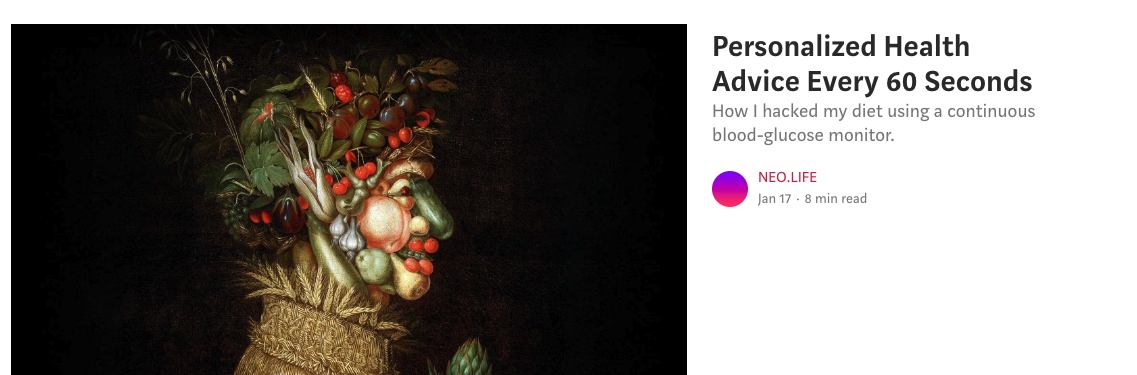
\includegraphics{images/sprague-neolife.png} Start with this article by \href{https://twitter.com/sprague}{Richard Sprague} at NEO.LIFE: \href{https://neo.life/2019/01/personalized-health-advice-every-60-seconds/}{``Personalized Health Advice Every 60 Seconds''}.

Also read this \href{https://medium.com/steady-health/the-ultimate-guide-to-continuous-glucose-monitors-cgm-611eecc70c9a}{good overview} by Henrik Berggren from Steady.Health.

\hypertarget{news-and-user-experiences}{%
\chapter{News and User Experiences}\label{news-and-user-experiences}}

\begin{itemize}
\item
  \textbf{New York Times Health Reporter Anahad O'Connor} wrote about Nutrisense, January.ai, and his personal experience using Levels Health. \url{https://www.nytimes.com/2021/02/08/well/diet-glucose-monitor.html}
\item
  \textbf{Lydia Ramsey}, senior reporter at Business Insider wrote a detailed summary of using a Dexcom G6: \url{https://www.businessinsider.com/what-its-like-to-track-blood-sugar-with-a-continuous-glucose-monitor-2019-11}
\item
  \textbf{Eric Jain} wrote a short, highly-readable account of his month-long experience: \url{https://eric.jain.name/2018/11/25/tracking-blood-sugar/}

  \begin{itemize}
  \tightlist
  \item
    And a \href{https://news.ycombinator.com/item?id=18891772}{Hacker News thread} about his post
  \end{itemize}
\item
  \textbf{Quantified Diabetes} does rigorous self-experimentation at \url{https://quantifieddiabetes.com/p/experiments.html}.\\
\item
  \textbf{Lily Nichols} is a registered dietitian who wrote ``\href{https://lilynicholsrdn.com/cgm-experiment-non-diabetic-continuous-glucose-monitor/}{What I Learned as a Non-Diabetic}''
\item
  \textbf{Jimi S,} a 25-year-old diabetic wrote a lengthy review: \href{https://medium.com/@JimiS/product-review-freestyle-libre-abbott-diabetes-care-561ee446eaa}{Review: FreeStyle Libre --- Abbott Diabetes Care \textbar{} by Jimi S.}
\item
  \textbf{``Quantified Bob'' Troia} wrote ``\href{https://www.quantifiedbob.com/measuring-glycemic-glucose-response-foods/}{How to measure personal glucose response to foods''}
\item
  \textbf{Jennifer Wang} writes ``Am I Crazy Because I Eat Too Much Sugar?'': \url{https://medium.com/@neogeo25/am-i-crazy-because-i-eat-too-much-sugar-a-cgm-experiment-5b310f334f10}
\item
  Follow Jessie Inchaspe's incredible Instagram account on her experiences with food and CGM: \url{https://www.instagram.com/glucosegoddess/}
\end{itemize}

\begin{figure}
\centering
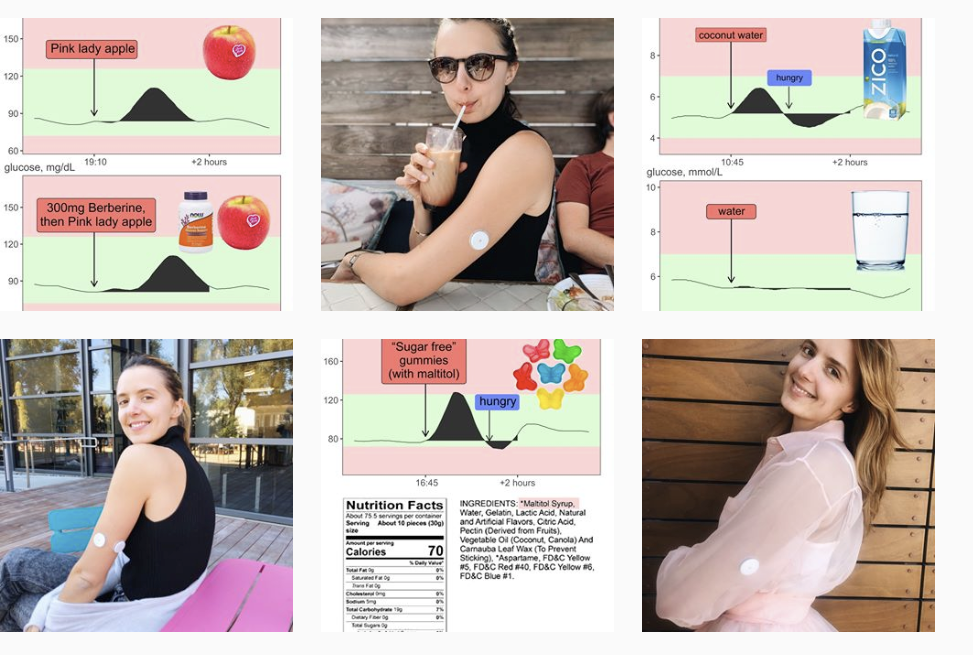
\includegraphics{images/glucose-goddess.png}
\caption{Glucose Goddess}
\end{figure}

\begin{itemize}
\tightlist
\item
  \textbf{Kevin Bass n-of-1}: A PhD student kept (2018-19) a\href{https://twitter.com/kevinstrials}{live Twitter feed} of his CGM data
\item
  \href{http://time.com/4703099/continuous-glucose-monitor-blood-sugar-diabetes/}{Why Perfectly Healthy People Are Using Glucose Monitors:}Time Magazine article from 2017
\item
  \href{https://news.ycombinator.com/item?id=15521882\#15522046}{Hacker News thread} about CGMs and sugar metabolism
\item
  \href{https://personalscience.shinyapps.io/librelink/}{Interactive web app} with daily updates from the Personal Science glucose monitor.
\item
  \href{https://imgur.com/a/2xNEgGA}{How accurate it is}: a user posts side-by-side comparisons of Freestyle Libre vs pinprick
\item
  \href{https://www.reddit.com/search?q=freestyle\%20libre}{Reddit forums} Lots of posts in diabetes-related forums
\end{itemize}

\href{http://abbott.mediaroom.com/2018-10-01-Abbott-s-FreeStyle-R-Libre-2-with-Optional-Real-Time-Alarms-Secures-CE-Mark-for-Use-in-Europe?fbclid=IwAR3B9sMnnUa44Aor42ctKUyAuUuG1ZLly3pnanVAAolX1PF6HRCV4SBaOyo}{Libre2 announcement} (Oct 2018)

\hypertarget{how-to-get-your-cgm}{%
\chapter{How to get your CGM}\label{how-to-get-your-cgm}}

The FreeStyle Libre is available over-the-counter at most pharmacies throughout the world (including Mexico and Canada), but requires a doctor's prescription in the United States.

A month's supply of sensors costs under US\$100, so don't bother trying to get your health insurance to reimburse you unless you have a specific medical reason, in which case consult your doctor.

There are three ways to get one in the US:

\begin{enumerate}
\def\labelenumi{\arabic{enumi}.}
\item
  Ask your doctor to prescribe one for you. The \href{https://www.freestylelibre.us/support/buying-guide.html}{Freestyle Buying Guide} gives detailed information about how the product works, and what to tell your doctor. Most doctors will be happy to prescribe it if you explain that you'll be paying out of pocket.
\item
  \href{https://tastermonial.com/products/cgm-freestyle-libre}{Tastermonial} will connect you with a doctor who can provide a prescription for \$29. This is the easiest solution for most people.
\item
  If you're traveling to Canada, Mexico, or other countries, you can pick them up locally, or you can order one to be shipped into the US. \href{https://octern.medium.com/how-to-get-a-continuous-glucose-monitor-d48cd229e9ac}{Michael Cohn} describes how he got one from Canada for about \$100
\end{enumerate}

\hypertarget{what-to-buy}{%
\section{What to buy}\label{what-to-buy}}

Buy the 14-day sensor by itself. If you have an iPhone 7 + or an Android, don't bother buying the Reader (which is an additional US\$200).

\hypertarget{companies-and-cgm-based-products}{%
\section{Companies and CGM-Based Products}\label{companies-and-cgm-based-products}}

Several companies will give you a month's worth of CGM with an app and nutrition advice for under \$500. See \protect\hyperlink{bookmark=id.d7g3e8qlegnl}{link below}.

\begin{figure}
\centering

\includegraphics{images/january-logo.png}
\caption{January, Inc.}
\end{figure}

\url{https://january.ai/} \$499 4-week program includes 2 Freestyle Libre devices and an app to guide your eating, fasting, and exercise choices.

\begin{figure}
\centering

\includegraphics{images/nutrisense-logo.png}
\caption{Nutrisense}
\end{figure}

\url{https://www.nutrisense.io/}: Join their ``cohort'' and receive 2 CGM devices/month and 24/7 nutritionist advice with an app that tracks your glucose, fasting, and more.

\begin{figure}
\centering

\includegraphics{images/steadyhealth-logo.png}
\caption{Steady Health}
\end{figure}

\url{https://steady.health/} a San Francisco-based clinic providing CGM-centric diabetes care. Their programs cost about \$60 / month and include AI-aided smartphone-based coaching and education around food and exercise, plus data interpretation with an endocrinologist. This is a good choice if your doctor has diagnosed you with diabetes.

\begin{figure}
\centering

\includegraphics{images/levelshealth-logo.png}
\caption{Levels Health}
\end{figure}

\url{https://www.levelshealth.com/} offers ``metabolic health'' services, including a CGM and nutritionist consultation for about \$400/month. You'll need to request access for a specific quote and availability.

\hypertarget{diet-and-food-tracking}{%
\chapter{Diet and food-tracking}\label{diet-and-food-tracking}}

Apps and websites useful for nutrition tracking

Bitesnap: take a photo of your food and get an AI-based identification, plus macronutrients and calories. Recognizes 1300+ foods.

https://getbitesnap.com/

LoseIt: Food database with 7 million+ foods, restaurant items and brands from around the world, hand curated by our on-staff nutrition experts.

https://www.loseit.com/

MyFitnessPal : 6 million foods, largest online community, connects to 50+ apps

\url{https://www.myfitnesspal.com/}

Cronometer

Large, curated food database. Widely used among professionals due to its in-depth tracking of nutrients and comprehensive data export.

\url{https://cronometer.com/}

\hypertarget{using-your-cgm-data}{%
\chapter{Using Your CGM Data}\label{using-your-cgm-data}}

Websites and apps that help you track glucose numbers.

\hypertarget{use-the-personal-science-app}{%
\section{Use the Personal Science App}\label{use-the-personal-science-app}}

The best way to analyze your CGM data is with the CGM app from Personal Science (makers of this web site). You can upload your data and study it for free here:

\url{https://cgm.personalscience.com}

\hypertarget{abbott-labs-official}{%
\section{Abbott Labs Official}\label{abbott-labs-official}}

The most important software for Freestyle Libre downloading is the officially-supported one here:

\url{https://provider.myfreestyle.com/freestyle-libre-resources.html}

Create an account on Libreview and then you can download your data as a CSV file here:

\url{https://www.libreview.com/meter}

\begin{figure}
\centering
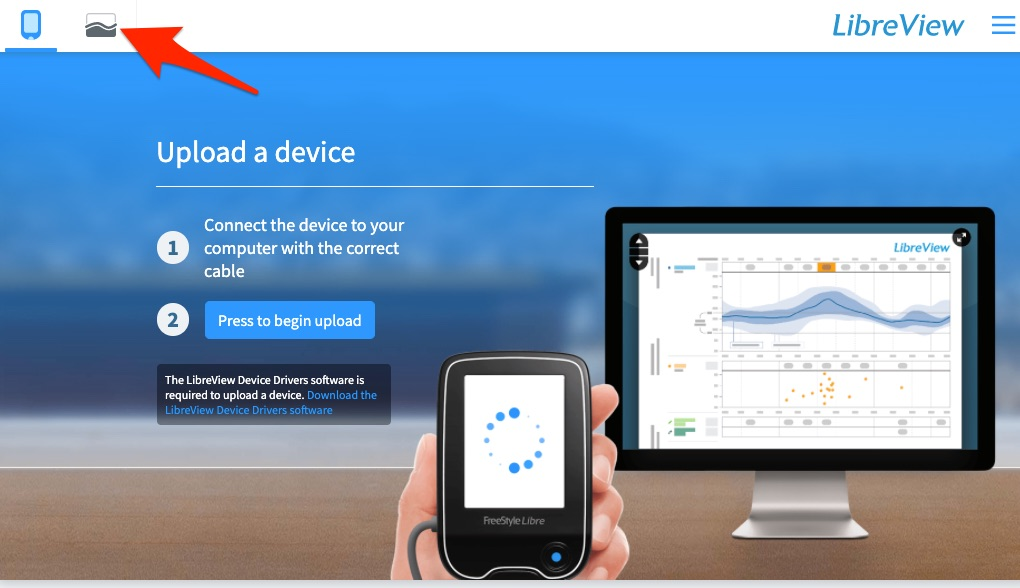
\includegraphics{images/freestyle-download.jpg}
\caption{Libreview main page}
\end{figure}

Then click here: \url{https://www.libreview.com/glucosereports}

\begin{figure}
\centering
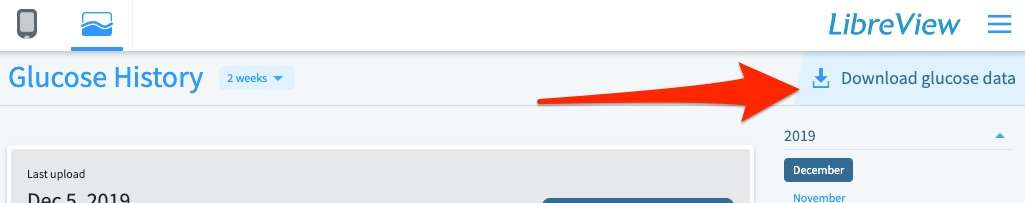
\includegraphics{images/freestyle-download-click.jpg}
\caption{Click to download}
\end{figure}

If you have the Abbott custom reader device, you can also download a Mac or Windows version of Freestyle Libre personal CGM

\begin{figure}
\centering
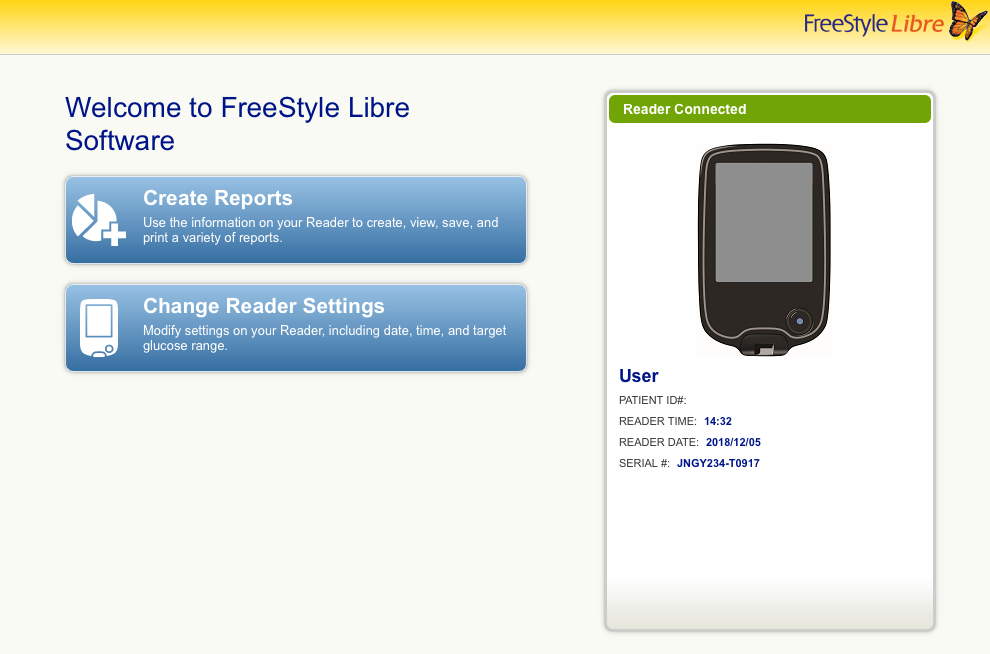
\includegraphics{images/freestyle-software.png}
\caption{Freestyle Libre Software}
\end{figure}

\hypertarget{international-versions}{%
\section{International versions}\label{international-versions}}

Freestyle Libre devices sold in other countries will generally work everywhere if you use the app downloaded specifically for that country.

This {[}table by \href{https://www.facebook.com/photo.php?fbid=1835069433269419\&set=gm.751003141928341\&type=3\&theater\&ifg=1}{Chuck Kub}{]} is a little old, but gives a sense of which models are available in which countries.

\textbf{China:} buy a reader plus 3 14-day sensor packs \href{https://item.jd.com/32498232197.html}{through Taobao} for about 1800 RMB (USD\$270)

\hypertarget{third-party}{%
\section{Third Party}\label{third-party}}

Many organizations now offer ways to upload and use your Freestyle (or other CGM) data.

Nightscout

``an open source, DIY project that allows real time access to a CGM data via personal website, smartwatch viewers, or apps and widgets available for smartphones''

See their app https://spike-app.com/

http://www.nightscout.info/

Diasend

(formerly called Glooko) tries to let you upload data from anywhere

https://diasend.com/us

Tidepool https://app.tidepool.org/patients

Open-source non-profit place to upload glucose data

https://tidepool.org

Diabetes:M

\url{https://diabetes-m.com/}

Glimp : popular Android app

https://play.google.com/store/apps/details?id=it.ct.glicemia

\hypertarget{open-source-software}{%
\chapter{Open Source Software}\label{open-source-software}}

\begin{itemize}
\tightlist
\item
  \textbf{Nightscout xDrip+}: \url{https://github.com/JoernL/xDrip-plus}

  \begin{itemize}
  \tightlist
  \item
    supports wireless connections to G4, G5, G6, Medtrum A6, Libre via NFC and Bluetooth, 630G, 640G, 670G pumps and Eversense CGM via companion apps. Bluetooth Glucose Meters such as the Contour Next One, AccuChek Guide, Verio Flex \& Diamond Mini as well as devices like the Pendiq 2.0 Insulin Pen
  \item
    44 contributors, very active since Nov 2014 (latest checkin Dec 2018)
  \item
  \end{itemize}
\item
  \textbf{OpenLibreReader} iOS: \url{https://github.com/blueToolz/openLibreReader-iOS-}

  \begin{itemize}
  \tightlist
  \item
    a project to connect the various Libre Transmitters to the iPhone.
  \item
    \href{https://unendlichkeit.net/wordpress/openlibrereader-and-status/?lang=en}{Blog post} (Jan 2018) summarizing goals and status.
  \item
    latest commit Apr 2018; Started in Nov 2017 by 2 Germans
  \end{itemize}
\item
  \url{https://github.com/UPetersen/LibreMonitor} iOS NFC reader, includes hardware instructions

  \begin{itemize}
  \tightlist
  \item
    last active: Nov 2018. Started in 2016 by 3 guys from Germany
  \end{itemize}
\item
  \textbf{nahog / freestyle-libre-parser-viewer: }\href{https://github.com/nahog/freestyle-libre-parser-viewer}{https://github.com/nahog/freestyle-libre-parser-v tiewer}

  \begin{itemize}
  \tightlist
  \item
    A parser library and viewer for CSV generated by the Abbott Freestyle Libre flash glucose meter.
  \item
    From 2016, last commit June 2018; One guy from Ireland
  \end{itemize}
\item
  \href{https://cran.r-project.org/web/packages/cgmanalysis/index.html}{cgmnalysis}: R Package on CRAN and \href{https://github.com/childhealthbiostatscore/R-Packages}{Github} cleans up data from multiple CGM devices

  \begin{itemize}
  \tightlist
  \item
    Last update October 2019
  \end{itemize}
\end{itemize}

\hypertarget{advanced-topics}{%
\chapter{Advanced Topics}\label{advanced-topics}}

\hypertarget{other-sites}{%
\section{Other Sites}\label{other-sites}}

Sites that are useful for general background

\begin{itemize}
\item
  \textbf{Abbott Freestyle Libre Users (Facebook):} \url{https://www.facebook.com/groups/748445301888935/}

  \begin{itemize}
  \tightlist
  \item
    Active (20K members) and includes people from Abbott
  \end{itemize}
\item
  \textbf{Diabettech site:} \url{https://www.diabettech.com/freestylelibre/}
\item
  \textbf{QS Guide: Testing Food with Blood Glucose: }another nice overview: \url{https://quantifiedself.com/blog/qs-guide-testing-food-with-blood-glucose/}
\item
  \textbf{Quantified Self Conference 2018} had a breakout session: see their notes here: \url{https://forum.quantifiedself.com/t/qs18-links-and-resources/5885/4} which are based on a lengthy \href{https://forum.quantifiedself.com/t/frequent-blood-sugar-measurement/3818}{May 2017 thread by Gary Wolf} in the same forum.
\item
  \textbf{Freestyle Libre Tips and Hacks}: Youtube videos by \href{https://www.youtube.com/channel/UC_20PWJ0X0HAloRioVvb5-A}{Nerdabetic}

  \url{https://www.youtube.com/watch?v=o7R5Of-iWfk}
\item
  \textbf{Reddit: /r/Diabetes}

  \begin{itemize}
  \tightlist
  \item
    Especially check the thread on \href{https://www.reddit.com/r/diabetes/comments/8axzlc/things_you_wished_you_knew_about_freestyle_libre/}{``Things you wished you knew about the Freestyle sensors''}
  \end{itemize}
\end{itemize}

\hypertarget{hardware}{%
\section{Hardware}\label{hardware}}

\hypertarget{freestyle-libre-hardware-information}{%
\subsection{Freestyle Libre hardware information}\label{freestyle-libre-hardware-information}}

\begin{itemize}
\tightlist
\item
  \href{http://idoroseman.com/freestyle-libre-blood-glucose-monitoring-system-teardown/}{Freestyle Libre sensor teardown}: Blogger Ido Roseman takes one apart, with photos.
\item
  Reddit forum \href{https://www.reddit.com/r/diabetes/comments/670qbw/librelink_and_the_s8/}{says}: ``it would appear that Libre sensors use NfcV, while S8 does not support NfcV (ISO 15693) but happily talks over NfcA and NfcB (ISO/IEC 14443). ``
\item
  Insulin calculator: settings/professional and password = CAA1C
\end{itemize}

\hypertarget{freestyle-compatible}{%
\subsection{Freestyle-compatible}\label{freestyle-compatible}}

Hardware devices that work with the Freestyle Libre. Using an NFC reader that talks directly to the Libre sensor, they send information to a bluetooth phone.

\begin{itemize}
\tightlist
\item
  \textbf{\href{https://miaomiao.cool/}{MiaoMiao}} Shanghai company \$200
\item
  \textbf{\href{https://www.ambrosiasys.com/}{Ambrosia Systems Nightrider}}: \$110 NFC-to-bluetooth device
\item
  \textbf{\href{https://www.bubblan.org/}{Bubblan}}: Supports All Libre Sensors except US Libre2 version : 139.99€
\end{itemize}

\hypertarget{other-hardware}{%
\subsection{Other hardware}\label{other-hardware}}

\begin{itemize}
\tightlist
\item
  \href{http://phware.com/Views/About.aspx}{Bionous}: Seattle-Bellevue company that claims to have a low-cost non-invasive glucose reader (PHWare)
\item
  \href{https://www.jobst-technologies.com/products/biosensors/}{Jobst Technologies Biosensors}: hardware company that sells biosensors that detect glucose.
\item
  \url{http://tula-health.com/content/tech.html} is raising money for a non-invasive CGM.
\item
  \href{https://docs.google.com/document/d/1ZyKx4_gGdBMYBQK0o32ftELf5tiShxAFo6mg1rph16U/edit\#}{OnDuo}: An open resource doc about Google-Verily and Sanofi's diabetes program that features CGM.
\item
  \href{https://docs.google.com/document/d/1sqmioRvVTh8XsljrLYUplDPhaTeehrJck0khOe6D-gI/edit\#}{Medtronic Guardian:} open resource doc about another sensor+phone integrated CGM with prediction capabilities
\end{itemize}

\hypertarget{scientific-articles}{%
\section{Scientific articles}\label{scientific-articles}}

\begin{itemize}
\tightlist
\item
  \href{https://journals.sagepub.com/doi/full/10.1177/1932296820958754}{Journal of Diabetes Science and Technology} (2020) concludes that Freestyle Libre 2 performs within 20\% of blood values.
\item
  \href{https://doi.org/10.1016/S0140-6736(16)31535-5}{Lancet article} (2016) that established the accuracy of the underlying CGM technology
\item
  \href{https://journals.plos.org/plosbiology/article/file?id=10.1371/journal.pbio.2005143\&type=printable}{Glucotypes} (2018): Stanford study claims people respond differently to foods

  \begin{itemize}
  \tightlist
  \item
    See news article \href{https://med.stanford.edu/news/all-news/2018/07/diabetic-level-glucose-spikes-seen-in-healthy-people.html}{summary}
  \item
    Upload your data to their online app here: \url{https://abreschi.shinyapps.io/shinySpecClust/}
  \end{itemize}
\item
  \href{https://www.cell.com/cell/fulltext/S0092-8674(15)01481-6?_returnURL=https\%3A\%2F\%2Flinkinghub.elsevier.com\%2Fretrieve\%2Fpii\%2FS0092867415014816\%3Fshowall\%3Dtrue}{Personalized Nutrition by Prediction of Glycemic Responses} (Cell: Zeevi et al 2015)

  \begin{itemize}
  \tightlist
  \item
    Highly-cited study showing differences are driven by the microbiome
  \end{itemize}
\item
  ``\href{https://www.ncbi.nlm.nih.gov/pmc/articles/PMC2769652/}{Continuous Gluose Profiles in Healthy Subjects}'' (2007) study.
\item
  \href{https://www.accessdata.fda.gov/cdrh_docs/pdf16/P160030S017a.pdf}{FDA approval document:} more details about Freestyle Libre and its authorized uses

  \begin{itemize}
  \tightlist
  \item
    (see \href{https://www.accessdata.fda.gov/cdrh_docs/pdf17/DEN170088.pdf}{similar approval} for Dexcom, a \emph{de novo} iCGM)
  \end{itemize}
\item
  \href{http://www.mendosa.com/The\%20Pursuit\%20of\%20Noninvsive\%20Glucose,\%20Fourth\%20Edition.pdf}{``Hunting the Deceitful Turkey''} 100+ page book about the tech behind non-invasive glucose monitoring
\end{itemize}

A handy table of CGM clinical trials (via \href{https://www.ajmc.com/journals/evidence-based-diabetes-management/2019/march-2019/continuous-glucose-monitoring-an-emerging-standard-of-care?p=2}{AMJC})

\begin{figure}
\centering
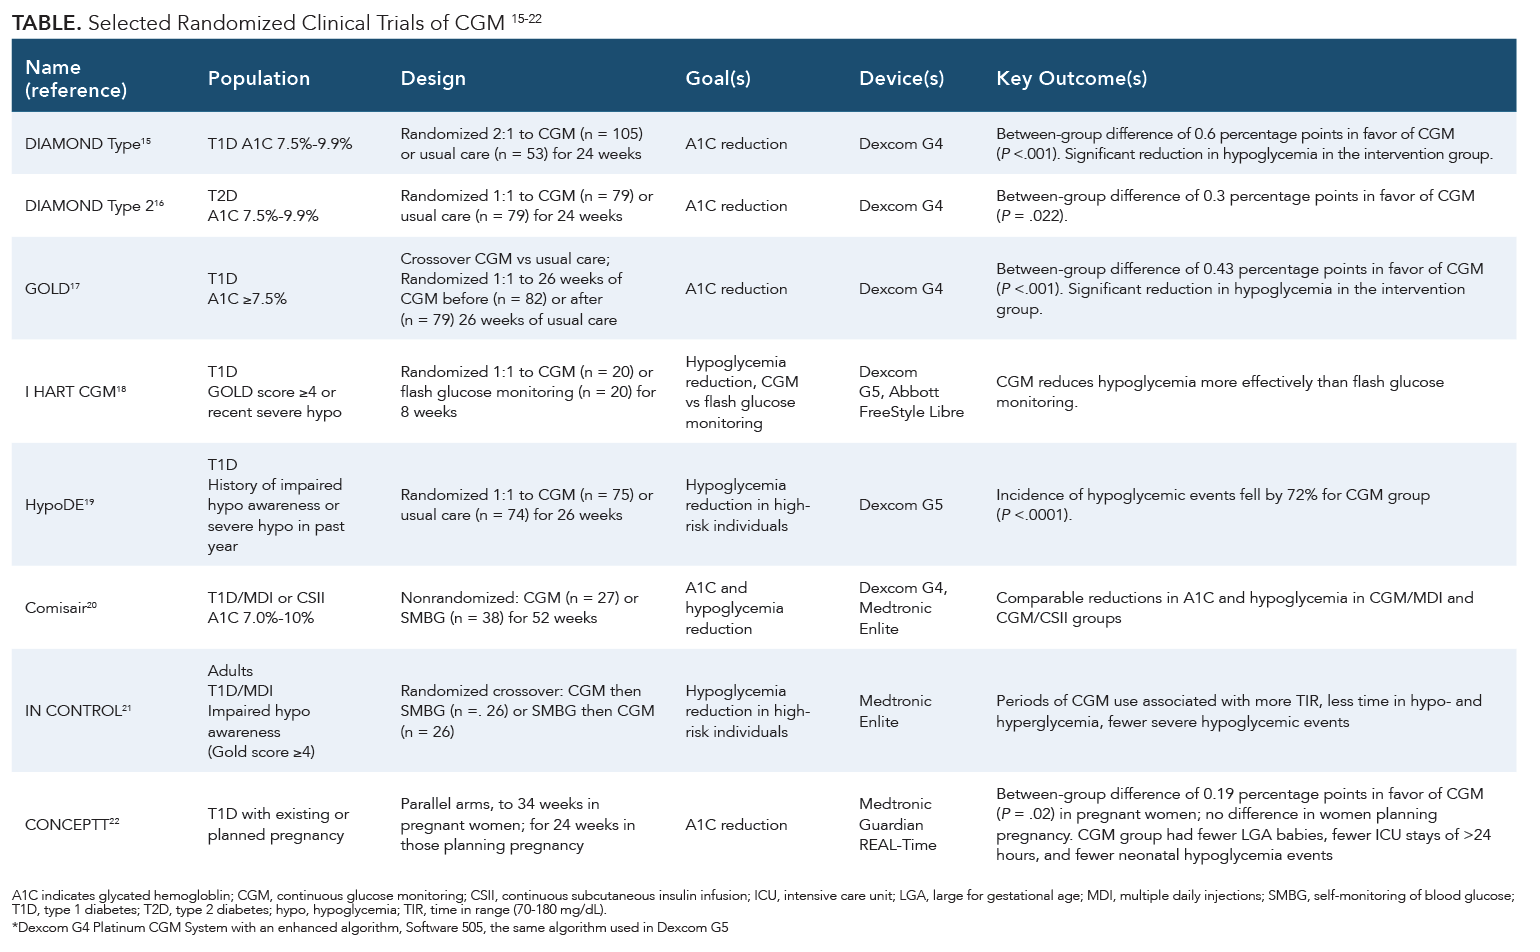
\includegraphics{images/AMJC-clinical-trials.png}
\caption{alt\_text}
\end{figure}

\hypertarget{other-summary-resources}{%
\chapter{Other Summary Resources}\label{other-summary-resources}}

Other places to find more links and other information

\href{https://loopkit.github.io/loopdocs/setup/requirements/cgm/\#continuous-glucose-monitor}{Continuous Glucose Monitor} page for the open source Loop project.

  \bibliography{book.bib,packages.bib}

\end{document}
